%File: formatting-instruction.tex
\documentclass[letterpaper]{article} %DO NOT CHANGE THIS
\usepackage{aaai19}  %Required
\usepackage{times}  %Required
\usepackage{helvet}  %Required
\usepackage{courier}  %Required
\usepackage{url}  %Required
\usepackage{graphicx}  %Required
\usepackage{amsmath}
\usepackage{mathrsfs}
\usepackage{color,soul}
\usepackage{listings}
\usepackage{caption,subcaption}
\usepackage{natbib}
\usepackage{multirow}
\usepackage{hhline}
\usepackage{mathrsfs}  
\usepackage{amsfonts}  



\newtheorem{mydef}{Definition}
\newtheorem{define}{Definition}


\newcounter{tmp}

% \usepackage{fontspec}
% \usepackage{unicode-math}
% \newcommand{\stripsp}{{\sc strips+}}
\newcommand{\stripsp}{{\sc STRIPS+}}
% \newcommand{\pddlthree}{{\sc PDDL3}}
\newcommand{\pddlthree}{{PDDL3}}
\newcommand{{\lama}}{{{LAMA}}}
\newcommand{\mercury}{{Mercury}}
\newcommand{{\fdss}}{{Fast Downward Stone Soup 2018}}
\newcommand{{\fdssshort}}{{FDSS 2018}}
\newcommand{\lamapruning}{$\text{LAMA}_{\text{P}}(h_\text{R})$}

\newcommand{{\miplan}}{{MIPlan}}
\newcommand{{\ibacop}}{{IBaCoP2}}
\newcommand{{\fdremixcomplete}}{{Fast Downward Remix}}
\newcommand{\lprpgp}{{LPRPG-P}}
\newcommand{{\fdremix}}{{FDRemix}}
% \newcommand{{\fifthIPC}}{{{IPC5}}}

\newcommand{\strips}{{\sc strips}}
\newcommand{\adl}{{\sc adl}}
\newcommand{\pddlIII}{{\sc{pddl3}}}
\newcommand{\stripspap}{{\sc strips+ap}}
\newcommand{\stripspp}{{\sc strips+p}}
\newcommand{\pddl}{{\sc pddl}}
% new command
\newcommand{\hplanp}{{HPlan-P}}
\newcommand{\mipsxxl}{{MIPS-XXL}}
\newcommand{\lpg}{{LPG}}
\newcommand{{\GBLcoles}}{{{GBL15-NB-B15}}}
% \newcommand{{\fifthIPC}}{{ {IPC5}}}
% \newcommand{{\fifthIPC}}{{\footnotesize {IPC5}}}
\newcommand{{\fifthIPC}}{{{IPC5}}}
\newcommand{\threatA}{T_{\mathcal{A}}(o)}
\newcommand{\violA}{V_{\mathcal{A}}(o)}
\newcommand{\threatSB}{T_{\mathcal{SB}}(o)}
\newcommand{\supportSB}{S_{\mathcal{SB}}(o)}
\newcommand{\threatAMO}{T_{\mathcal{AO}}(o)}
\newcommand{\supportST}{S_{\mathcal{ST}}(o)}
\newcommand{\affected}{\mathcal{I}(o)}
\newcommand{\truettt}{\small \texttt{TRUE}}
\newcommand{\pviol}{P\textit{-violated}}
\newcommand{\affectedd}{P_{\textit{affected}}(o)}

\frenchspacing  %Required
\setlength{\pdfpagewidth}{8.5in}  %Required
\setlength{\pdfpageheight}{11in}  %Required
%PDF Info Is Required:
  \pdfinfo{
/Title (Compiling PDDL3 Qualitative Preferences without Using Automata)
/Author (Anonymous)}
\setcounter{secnumdepth}{0}  
 \begin{document}
% The file aaai.sty is the style file for AAAI Press 
% proceedings, working notes, and technical reports.
%
\title{Compiling PDDL3 Qualitative Preferences without Using Automata}
\author{...
}
\maketitle
\begin{abstract}
We address the problem of planning with preferences in propositional 
domains extended with the class of (preferred) temporally extended goals 
supported in  {\pddlIII}, that is part of the standard planning language 
{\pddl} since the 5th International Planning Competition (\fifthIPC). Such 
preferences are useful to characterise plan quality by allowing the user
to express certain soft constraints on the state trajectory of the desired
solution plans.
Starting from the work of Keyder and Geffner on compiling (reachability)
soft goals, we propose a compilation scheme
for translating a {\strips} problem enriched with qualitative  {\pddlIII}
preferences  (and possibly also with soft goals) into an equivalent {\strips}
problem with action costs. 
The proposed compilation, which supports all types of preferences in the benchmarks
from \fifthIPC, allows many existing {\strips} planners to immediately address
planning with preferences. 
An experimental analysis presented in the paper evaluates the performance of
state-of-the-art {\strips} planners supporting action costs using our compilation
approach to deal with qualitative  {\pddlIII} preferences.  The results indicate
that our approach is highly competitive with respect to current planners that
natively support the considered class of preferences.
\end{abstract}



%%%%%%%%%%%%%%%%
% INTRODUZIONE %
%%%%%%%%%%%%%%%%
\section{Introduction}
Planning with preferences, also called ``over-subscription planning" in \cite{Briel-et-al:AAAI04,do-kambhampati04,smith04}, concerns the generation of plans for problems involving soft goals or soft state-trajectory constraints (called preferences in \pddlIII), that it is desired a plan satisfies, but that do not have to be satisfied. The quality of a solution plan for these problems depends on the soft goals and preferences that are satisfied.

For instance, a useful class of preferences than can be expressed in {\pddlIII} \cite{GHLS+09} consists of  {\em always preferences}, requiring that a certain condition should hold in {\em every} state reached by a plan. As discussed in \cite{Weld:94AA,bacKab,GHLS+09,Hplanp:aij09}, adding always preferences to the problem model can be very useful to express safety or maintenance conditions, and other desired plan properties. An simple example of such conditions is ``whenever a building surveillance robot is outside a room, all the room doors should be closed". 

{\pddlIII} supports other useful types of preferences, and in particular the qualitative preferences of types {\em at-end}, which are which are equivalent to soft goals, {\em sometime}, {\em sometime-before} and  {\em at-most-once}, which are all the types used in the available benchmarks for planning with qualitative {\pddlIII} preferences \cite{GHLS+09}. Examples of preferences that can be expressed  through these constructs in a logistics domain are: ``sometime during the plan the fuel in the tank of every vehicle should be full'', ``a certain depots should be visited before another once'',  ``every store should be visited at most once'' (the reader can find additional examples in \cite{GHLS+09}).
 
In this paper, we study propositional planning with these types of preferences through a compilation approach. 




%%%%%%%%%%%%%%%%
% RELATED WORK %
%%%%%%%%%%%%%%%%
\section{Related Work}
Our compilative approach is inspired by the work of Keyder and Geffner \cite{kn:geffner09}
on compiling soft goals into {\strips} with action costs (here denoted with \stripsp). In this work
the compilation scheme introduces, for each soft goal $p$ of the problem, a dummy goal $p'$ that
can be achieved using two actions in mutual exclusion. The first one, which is called \textit{collect(p)},
has cost equal to 0 and requires that $p$ be true when it is applied; the second one, whic is called \textit{forgo(p)},
has cost equal to the utlity of $p$ and requires that $p$ be false when it is applied.
\\\indent Both of these action can be performed at the end of the plan and for each soft goal $p$ but just one of
$\{$\textit{collect(p), forgo(p)}$\}$ can appear in the plan depending on whether the soft goal
has been achived or not. This scheme has achieved good perfomance which can be improved with the use of
an ad hoc admissible heuristic based on the reachability of soft goals \cite{percassi2017improving}.

The most prominent existing planners supporting {\pddlIII} preferences are {\hplanp} \cite{Hplanp:aij09,BM:AAAI06},
which won the ``qualitative preference" track of IPC-5, {\mipsxxl} \cite{Edelk06,Edelk} and the more recent {\lprpgp} \cite{LPRPGP-P:icaps11}
and its extension in \cite{coles2013searching}.
%
These (forward) planners represent preferences through automata whose states are synchronised with the states generated by the action plans, so that an accepting automaton state corresponds to preference satisfaction. For the synchronisation, {\hplanp} and {\lprpgp} use planner-specific techniques, while {\mipsxxl} compiles the automata by modifying the domain operators and adding new ones modelling the automata transitions of the grounded preferences. 

Our computation method is very different from the one of {\mipsxxl} since, rather than translating automata into new operators, the problem preferences are compiled by only modifying the domain operators, possibly creating multiple variants of them. Moreover, our compiled files only use {\stripsp}, while {\mipsxxl} also uses numerical fluents.\footnote{Another compilation scheme using numerical fluents is considered in \cite{GHLS+09} to study the expressiveness of \pddlIII (without an implementation).}

The works on compiling LTL goal formulas by Cresswell and Coddington \cite{CC:ECAI04} and Rintanen \cite{Rintanen:ECAI00}
are also somewhat related to ours, but with important differences. Their methods handle {\em hard} temporally extended
goals instead of preferences, i.e., every temporally extended goal must be satisfied in a valid plan, and hence there
is no notion of plan quality referred to the amount of satisfied preferences. Rintanen's compilation considers only
single literals in the always formulae (while we deal with arbitrary CNF formulas), and it appears that extending
it to handle more general formulas requires substantial new techniques \cite{Rintanen:personal2015}. 
An implementation of Crosswell and Coddington's approach is unavailable, but Bayer and McIlaraith \cite{BM:AAAI06} observed
that their approach suffers exponential blow up problems and performs less efficiently than the approach of {\hplanp}.

\hl{IMPORTANTE, CONFRONTO LAVORO NEBEL:} An important work about soft-trajectory constraints compilation,
which is closely related to ours, has been recently proposed by Wright, Matt\"uller and
Nebel in \cite{nebelCompiling} (cerca riferimento articolo Nebel). This approach is a based
on the compilation of the soft trajectory constraints into conditional effects and state dependent action costs using
$\sf{LTL}_{\text{f}}$ and B{\"u}chi automata. There are some similarities between  
between our and their approach but at the same time there are also
differences. 

\textbf{FP: differenze approccio Nebel e nostro: 1) numero di fluenti introdotto nella compilazione diverso; 2) il nostro
e' un approccio piu' specifico PDDL3-oriented, il loro piu' generale; 3) diverso meccanismo di aggiornamento dei costi, nel loro caso
ricompensa e penalita', nel nosto solo penalità 4) il loro schema prevede quindi costi negativi e postivi, il nostro positivi; nel loro caso per avere solo costi positivi e' necessario perdere l'ottimalita' nel nostro caso no ed inoltre volendo potremmo introdurre dei costi
negativi per quelle preferenze la cui violazione puo' essere testata solo alla fine del piano mantenendo l'ottimalita'; ho fatto inoltre menzione del fatto che i costi possono essere incrementanti il prima possibile (es. always)}

\textbf{1)} In our approach, given a preference $P$,
we introduce at most a pair of boolean fluents, typically one additional fluent to 
represent if a preference is violated or not ($P\textit{-violated}$) and
in some cases an additional fluent to correctly represent the status of a preference during
the planning,
while in their approach it is introduced a boolean variable
for each state of the corresponding automaton of $P$. \textbf{2)} Their approach is more general
while ours is focused on PDDL3 constraints and therefore it is more specific.

\textbf{3)} In their work the cost of the plan during the planning is updated by using rewards
and penalties (negative and positive costs respectively). The cost of the plan is increased whenever
a violation of a preference (also reversible) occurs. On the contrary,
if an operator causes the satisfaction of a preference then the cost of the plan is decreased.
In both cases the negative or positive cost is equal to the utility of the interested preference\footnote{
\hl{Messo in footnote altrimenti era troppo lungo:}
Note that 
both the violation and the satisfaction of a preference may be temporary conditions depending on the type 
of interested preference. For example an always preference can be irreversibly violated and its satisfaction can only be evaluated at the end of the plan considering the whole trajectory of the states; on the contrary a sometime-after preference can be satisfied and violated several times during the execution of the plan.
}. \textbf{4)} This type of cost update requires the use of negative costs while our compilation scheme produces a problem
whose costs are monotonically increasing because, similarly to what was proposed in Keyder and Geffner,
costs are realized only at the end of the planning. In our scheme some costs can be anticipated for those preferences whose violation is irreversible (e.g. always, sometime-before) and negative costs could be used for those preferences that may be ``temporarily" violated (e.g. sometime, at-end). In both cases our scheme would maintain the optimality but in this work we have provided a compilation based only on positive costs in order to take advantage of a wider spectrum of classical planners (few planners still support negative costs).








we propose a compilation scheme for translating a {\strips} problem with {\pddlIII} qualitative preferences into an equivalent {\stripsp} problem. Handling action costs is a practically important, basic functionality that is supported by many powerful planners; the proposed compilation method allows them to immediately support (through the compiled problems)  the considered class of preferences with no change to their algorithms and code.


%%%%%%%%%%%%%%%%%%%%%%%%%%%%%%%%
% SEZIONE DEFINIZIONE PROBLEMA %
%%%%%%%%%%%%%%%%%%%%%%%%%%%%%%%%
\section{Propositional Planning with Qualitative PDDL3 Preferences}
A {\strips}  problem is a tuple $\langle F, I, O, G\rangle$ where $F$ is a set of fluents, $I \subseteq F$ and $G \subseteq F$ are the initial state and goal set, respectively, and $O$ is a set of actions or operators defined over $F$ as follows.

A {\strips} operator $o \in O$ is a pair $\langle \textit{Pre}(o), {\textit{Eff}}(o)\rangle$, where 
$\textit{Pre}(o)$ is a sets of atomic formulae over $F$ and ${\textit{Eff}}(o)$ is a set of literals over $F$.  ${\textit{Eff}}(o)^+$ denotes the set of positive literals
in ${\textit{Eff}}(o)$, ${\textit{Eff}}(o)^-$ the set of negative literals in ${\textit{Eff}}(o)$.
An action sequence $\pi=\langle a_0, \ldots, a_m\rangle$ is applicable in a planning problem $\Pi$ if all actions $a_i$ are in $O$ and there exists a sequence of states $\langle s_0, \ldots, s_{m+1}\rangle$ such that $s_0=I$, $prec(a_i) \subseteq s_i$ and $s_{i+1}=s_i  \setminus 
\{p \mid \neg{p} \in {\textit{Eff}}(a_i)^-$\}$\cup{\textit{Eff}}(a_i)^+$, for $i = 0 \dots m$. Applicable action sequence $\pi$ achieves a fluent $g$ if $g \in s_{m+1}$, and is a valid plan for $\Pi$ if it achieves each goal $g \in G$ (denoted with $\pi \models G$).

A {\stripsp} problem is a tuple $\langle F,I,O,G,c \rangle $, where $\langle F,I,O,G \rangle $ is a {\strips} problem and $c$ is a function 
mapping each $o\in O$ to a non-negative real number.
The cost $c(\pi)$ of a plan $\pi$ is $\sum_{i=0}^{|\pi|-1} c(a_i)$, where $c(a_i)$ denotes the cost of the $i$th action $a_i$ in $\pi$ and $|\pi|$ is the length of $\pi$.

Starting from a {\stripsp} problem we define the 
notion of state trajectory generatered by a plan. Given a 
{\stripsp} $ \Pi = \langle F,I,O,G,c \rangle $ problem, a plan $\pi$ generates the trajectory
$\langle (S_0,0),(S_1,t_1),...,(S_n,t_n)\rangle$ iif
$S_0 = I$ and for each happening $h$ generated by $\pi$, with $h$
at time $t$, there is some $i$ such that $t_i = t$ and $S_i$ is the
result of applying the happening $h$ to $S_{i-1}$, and for every
$j \in \{1 \ldots n\}$ there is a happening $\pi$ at $t_j$.

The following is a fragment of the grammar of {\pddlIII},
describing the new modalities of {\pddlIII} for expressing these soft state-trajectory constraints
(indicated with {\small \texttt{con-GD}})
(the full BNF grammar is given in \cite{techReportGerevini1,techReportGerevini2})
where \texttt{<GD>} is a goal description (a first order logic formula):

{\small
\begin{verbatim}
  <con-GD> ::= (at end <GD>) | (always <GD>) |
               (sometime <GD>) |
               (at-most-once <GD>) | 
               (sometime-after <GD> <GD>) | 
               (sometime-before <GD> <GD>)
\end{verbatim}
}
Let $\phi$ and $\psi$ be atomic formulae over the predicates of a planning problem,
then interpretation of the modal operators considered in this work is specified in Figure \ref{fig:semantics} [COMMENTATA].
We write $\pi \models P$ to indicate that the state-trajectory generated by $\pi$ satisfies a preference $P$ and we indicate with $\mathcal{A}$, $\mathcal{SB}$, $\mathcal{ST}$, $\mathcal{AO}$, $\mathcal{SG}$ the classes of all preferecense of always, sometime-before, sometime, at-most-once and soft goal respectively for a given {\stripsp} problem.


% FIGURA CONTENENTE LA SEMANTICA DA SCOMMENTARE

% \begin{figure}[t]
% \vspace{-7mm}
% {\small
% \[\begin{array}{ll}
% \multicolumn{2}{l}{\langle (S_0,0),(S_1,t_1),...,(S_n,t_n)\rangle \models (\mbox{\textit{at\,end}}~\phi)} \\
%  & \hspace{1cm} \mbox{iff} \hspace{5mm} S_n \models \phi\\
% \multicolumn{2}{l}{\langle (S_0,0),(S_1,t_1),...,(S_n,t_n)\rangle \models \phi} \\
%  &\hspace{1cm}  \mbox{iff} \hspace{5mm} S_n \models \phi\\
% \multicolumn{2}{l}{\langle (S_0,0),(S_1,t_1),...,(S_n,t_n)\rangle \models (\mbox{\textit{always}}~\phi)} \\
%   &\hspace{1cm} \mbox{iff} \hspace{5mm} \forall i: 0 \leq i\leq n \cdot S_i \models \phi\\
% \multicolumn{2}{l}{\langle (S_0,0),(S_1,t_1),...,(S_n,t_n)\rangle \models (\mbox{\textit{sometime}}~\phi)} \\
%  &\hspace{1cm}  \mbox{iff} \hspace{5mm} \exists i: 0 \leq i \leq n \cdot S_j \models \phi\\

% \multicolumn{2}{l}{\langle (S_0,0),(S_1,t_1),...,(S_n,t_n)\rangle \models (\mbox{\textit{at-most-once}}~\phi)}\\
% &\hspace{1cm}  \mbox{iff} \hspace{5mm} \forall i : 0 \leq i \leq n \cdot~\mbox{if}~S_i \models \phi~\mbox{then}~\\
% &\hspace{3.8cm} \exists j : j \geq i \cdot \forall k : i \leq k \leq j \cdot S_k \models \phi \mbox{ and}~\\
% &\hspace{3.8cm} \forall k : k > j \cdot S_k \models \neg\phi\\

% \multicolumn{2}{l}{\langle (S_0,0),(S_1,t_1),...,(S_n,t_n)\rangle \models
% (\mbox{\textit{sometime-after}}~\phi~\psi)}\\
%  & \hspace{1cm} \mbox{iff} \hspace{5mm} \forall i \cdot 0 \leq i \leq n \cdot \mbox{if}~S_i \models \phi~\mbox{then}~\exists j : i \leq j \leq n \cdot S_j \models \psi \\
% \multicolumn{2}{l}{\langle (S_0,0),(S_1,t_1),...,(S_n,t_n)\rangle \models
% (\mbox{\textit{sometime-before}}~\phi~\psi)}\\
%  & \hspace{1cm} \mbox{iff} \hspace{5mm} \forall i \cdot 0 \leq i \leq n \cdot \mbox{if}~S_i \models \phi~\mbox{then}~\exists j : 0 \leq j < i \cdot S_j \models \psi \\

% \end{array}\]
% }

% \vspace{-0.5cm}
% \caption{\label{fig:semantics}
% Semantics of the basic modal operators in {\pddlIII}. $\phi$ and $\psi$ stand for arbitrary (syntactically valid) goal formulae of {\pddlIII}.}
% \end{figure}

But in the following, without loss of generality, we will assume in the discussion that the formula $\phi$ and $\psi$ involved in a preference $P$ is expressed in conjuctive normal form $\phi = \phi_{1} \land \phi_{2} \land ... \land \phi_{n}$ where each $\phi_{i}$ ($i \in \{1 \ldots n\}$) is a clause of $P$ formed by literals over the problem fluents. 

\begin{mydef}
A {\strips+} problem with preferences is a tuple $\langle F, I, O, G, \mathscr{P}, c, u \rangle$ where:
\begin{itemize}
    \item $\langle F,I,O,G,c \rangle$ is a \strips+ problem;
    \item $\mathscr{P} = \{ \mathscr{P}_{\mathcal{A}}  \cup  \mathscr{P}_{\mathcal{SB}} \cup  \mathscr{P}_{\mathcal{ST}} \cup  \mathscr{P}_{\mathcal{AO}} \cup  \mathscr{P}_{\mathcal{SG}} \}$ is the set of the preferences of\ $\Pi$ where $\mathscr{P}_{\mathcal{A}} \subseteq \mathcal{A}$, $\mathscr{P}_{\mathcal{SB}} \subseteq \mathcal{SB}$, $\mathscr{P}_{\mathcal{ST}} \subseteq \mathcal{ST}$, $\mathscr{P}_{\mathcal{AO}} \subseteq \mathcal{AO}$ and $\mathscr{P}_{\mathcal{SG}} \subseteq \mathcal{SG}$;
    \item $u$ is an utility function mapping each $P \in \mathscr{P}$ to a value in $\mathbb{R}_0^{+}$.
\end{itemize}
\end{mydef}

In the following the class of {\stripsp} problems with a set of preferences is indicated with \stripspp.

\begin{mydef}
Let $\Pi$ be a {\stripspp} problem. The utility $u(\pi)$ of a plan $\pi$ solving $\Pi$ is the difference between the total amount of utility of the preferences by the plan and its cost:
$$u(\pi) = \sum_{P \in \mathscr{P}: \pi \models_{} P}{u(P)} - c(\pi).$$
\end{mydef}

The definition of plan utility for {\stripspp} is similar to the one given for {\stripsp} with soft goals by Keyder and Geffner \cite{kn:geffner09}. 
A plan $\pi$ with utility $u(\pi)$ for a {\stripspp} problem is optimal when there is no plan $\pi'$ such that $u(\pi') > u(\pi) $. The definitions below are introduced to simplify the notation in the discussion.

\section{Operator-Preference Interactions}

The definitions below are introduced to simplify the notation in the discussion.

\begin{mydef}
Given a preference clause $\phi_{i} = l_1 \lor l_2 \lor ... \lor l_m$, the set $L(\phi_{i}) = \{l_1, l_2, ..., l_m\}$ is the equivalent set-based definition of $\phi_{i}$ and $\overline{L}(\phi_{i}) = \{\lnot l_1, \lnot l_2, ..., \lnot l_m\}$ is the literal complement set of $L(\phi_{i})$.
\end{mydef}

\begin{mydef}
Given an operator $o \in O$ of a {\stripspp} problem, $Z(o)$ is the set of literal defined as:
$$
Z(o) = (\textit{Pre}(o) \setminus \{p \mid \lnot p \in \textit{Eff}(o)^{-}\}) \cup \textit{Eff}(o)^{+} \cup \textit{Eff}(o)^{-}.
$$
\end{mydef}
Note that the literals in $Z(o)$ hold in any reachable state resulting from the execution of operator $o$.

To shorten the following definitions and explanation we indicate the state where the operator $o$ is applied with $s$ and the state resulting from the application of $o$ with $s'$.

\begin{mydef}\label{def:trueclauses}
Given an operator $o$ and CNF formula $\phi = \phi_{1} \land ... \land \phi_{n}$, we define the set of clauses which will surely be true
in the resulting state from the application of $o$ as:
% $$
% C_{\phi}(o) =  \{\phi_{i} \mid L(\phi_{i}) \cap Z(o) \not = \O, \;i \in \{1 \ldots n\}\}
% $$
$$
C_{\phi}(o) =  \{\phi_{i} : |L(\phi_{i}) \cap Z(o)| > 0, \;i \in \{1 \ldots n\} \}
$$
We can also define the complementary set of the remaining clauses of $\phi$ which does not satisfy the previous condition as $\overline{C}_{\phi}(o) = \{ \phi_{i} : \phi_i \not \in C_{\phi}(o), \;i \in \{1 \ldots n\} \}$
\end{mydef}

\begin{mydef}
Given a preference clause $\phi_{i} = l_1 \lor l_2 \lor ... \lor l_m$, the set $L(\phi_{i}) = \{l_1, l_2, ..., l_m\}$ is the equivalent set-based definition of $\phi_{i}$ and $\overline{L}(\phi_{i}) = \{\lnot l_1, \lnot l_2, ..., \lnot l_m\}$ is the literal complement set of $L(\phi_{i})$.
\end{mydef}

\begin{mydef}
Given an operator $o \in O$ of a {\stripspp} problem, $Z(o)$ is the set of literal defined as:
$$
Z(o) = (\textit{Pre}(o) \setminus \{p \mid \lnot p \in \textit{Eff}(o)^{-}\}) \cup \textit{Eff}(o)^{+} \cup \textit{Eff}(o)^{-}.
$$
\end{mydef}
Note that the literals in $Z(o)$ hold in any reachable state resulting from the execution of operator $o$.

To shorten the following definitions and explanation we indicate the state where the operator $o$ is applied with $s$ and the state resulting from the application of $o$ with $s'$.

\begin{mydef}\label{def:trueclauses}
Given an operator $o$ and CNF formula $\phi = \phi_{1} \land ... \land \phi_{n}$, we define the set of clauses which will surely be true
in the resulting state from the application of $o$ as:
% $$
% C_{\phi}(o) =  \{\phi_{i} \mid L(\phi_{i}) \cap Z(o) \not = \O, \;i \in \{1 \ldots n\}\}
% $$
$$
C_{\phi}(o) =  \{\phi_{i} : |L(\phi_{i}) \cap Z(o)| > 0, \;i \in \{1 \ldots n\} \}
$$
We can also define the complementary set of the remaining clauses of $\phi$ which does not satisfy the previous condition as $\overline{C}_{\phi}(o) = \{ \phi_{i} : \phi_i \not \in C_{\phi}(o), \;i \in \{1 \ldots n\} \}.$
\end{mydef}

With reference to Definition \ref{def:trueclauses}, given a clause $\phi_{i} = l_1 \lor ... \lor l_{m_i}$ of $\phi$, the condition $|L(\phi_{i}) \cap Z(o)| > 0$ requires that exists at least a literal $l_j$, with $j \in \{1 \ldots m_i\}$, that, belonging to the set $Z(o)$, will be certainly true in the resulting state from the application of the operator $o$ thus making the clause $\phi$ true in $s'$.

% Each literal $l_j \in Z(o)$ can be true in $s'$ in different ways: \textit{i)} it could be already true in the preconditions of $o$, so in $s$, and not falsified by $o$ or \textit{ii)} it could become true in $s'$ by the effects of $o$ regardless of whether it was true or false in $s$.

\begin{mydef}\label{def:becometrue}
Given an operator $o$ and a CNF formula $\phi = \phi_{1} \land ... \land \phi_{n}$, we say that $o$ \textbf{can make true} $\phi$ if
\begin{enumerate}
% $C_{\phi}(o) \not = \O$ and
\item $|C_{\phi}(o)|>0$;

\item for each clause $\phi \not \in \overline{C}_{\phi}(o), \; \overline{L}(\phi) \not \subseteq Z(o)$.

\end{enumerate}
\end{mydef}

The first condition in Definition \ref{def:becometrue} requires that exists at least a clause of the formula which contains some literals which will certainly be true true in the state resulting from the execution of $o$. The second condition in Definition \ref{def:becometrue} requires that the remaining clauses of $\phi$, which do not belong to $C_{\phi}(o)$, are certainly not falsified in $s'$, because otherwise the $\phi$ formula will be certainly falsified in $s'$.

An operator $o$ that \textit{can make} $\phi$ does not not guarantees a switch from a state $s \models \lnot \phi$ to a state $s' \models \phi$, but it only guarantees $s' \models \phi$ without imposing any condition on the truth value of $\phi$ in $s$.

In our compilation scheme of a {\stripspp} problem we have to distinguish, for each kind of preference,
different class of operators in order to specialize the operators compilation based on 
how they interact with the preferences of the problem.

Generally speaking, we can identify three classes of operators regardless of the type of preference considered. An
operator is a \textit{threat} for a preference $P$ if in case it is executed it may violate $P$. An
operator is a (potential) \textit{support} for a preference $P$ if in case it is executed it could satisfy $P$. Finally,
an operator $o$ is \textit{neutral} for a preference $P$ if its execution
can not influence the current state of the preference. In the following Subsection \ref{subsection:always_operators}--\ref{subsectionAMO}
we will decline these generic definitions of classes of operators for each type 
of considered preference providing for each of them a formal definition.

In the following definitions of operators classes we will assume that $\phi$ (and $\psi$ in the case of dual preferences) are arbitrary CNF formulae $\phi = \phi_{1} \land ... \land \phi_{n}$ where each clause $\phi_{i} = l_{1} \lor ... \lor l_{m_{i}}$ for each $i \in \{1 \ldots n\}$.

\section{Compilation of Qualitative Preferences}



% EXPERIMENTAL RESULTS
\section{Experimental Results}

\subsection{Experiments Description}


We implemented the proposed compilation scheme and have evaluating it
by two sets of experiments with different purposes. On the one hand we
evaluated the scheme in a satisficing planning context in which we focused
on the search for sub-optimal plans using different planning systems,
while in the other we focuse on the
search of optimal plans using admissible heuristics.

Regarding the comparison in the context of the satisficing planning
we have considered the following {\stripsp} planning system
{\lama}\cite{RicLAMA}, {\mercury} \cite{MercuryIPC8},
{\miplan} \cite{nunez2014miplan}, {\ibacop} \cite{cenamor2014ibacop}, which are some of the best
performing planning system in IPC8 \cite{vallati20152014}, and
\fdss \cite{fdss2018}, \fdremixcomplete \cite{fdremix} (abbreviated with \fdremix),
which are some of the best performing planning system in the last IPC9 \cite{ipc9website}
which have been compared with {\lprpgp} \cite{coles2011lprpg}, which is one of the
performing planner which supports PDDL3 preferences. Moreover have considered our 
specifically enhanced version of {\lama} for planning with soft goal,
which is {\lamapruning}, which makes use of admissibile
heuristic $h_\text{R}$ to test the reachability of the soft goals
of the problem \cite{percassi2017improving}.

As benchmark we have considered the five domains 
of the qualitative preference track of IPC5 \cite{GHLS+09}
which involve always, sometime, sometime-before, at-most-once and soft goal preferences, i.e
Rovers, TPP, Trucks, Openstacks and Storage. 

For each original 
problem all preferences and each original utility were kept. The 
the classical planners were runned on the compiled problems while {\lprpgp}
was runned on the original problems of the competition. All the experiments
were conducted on a 2.00GHz Core Intel(R) Xeon(R) CPU E5-2620 machine with CPU-time
and memory limits of 30 minutes and 8GiB, respectively, for
each run of every tested planner. We have tested 8 planners for 5 domains
each of which consists of 20 instances for a total of 800 runs.

Table \ref{tab:ipc_score} shows the performances of the considered planning system
in term of plans quality. As quality measure we have used the IPC quality score, a
popular metric of which we have reported a brief description \cite{IPC6}. 

Given a planner $p$ and a task $i$ we assign, if $p$ solves $i$, the
following score to $p$:
$$
% \textit{score}(p, i) = \textit{cost}_{\textit{best}} (i) / \textit{cost}(p, i)
\textit{score}(p, i) = \frac{\textit{cost}_{\textit{best}} (i)}{\textit{cost}(p, i)}
$$

where $\textit{cost}_{\textit{best}}(i)$ is the cost of the best know
solution for the task $i$ 
found by any planner, and $\textit{cost}(p, i)$
is the cost of the solution found by the considered planner $p$ in 30 minutes. In our 
case our reference for $\textit{cost}_{\textit{best}} (i)$ is equal to the
cost of the best solution among the tested planners within 30 minutes. If $p$
did not find a solution within the time assigned, then $\textit{score}(p, i)$
is equal to $0$ in order to reward both quality and coverage. 

The quality score assigned to each tested planner $p$ is set equal to 
sum of the quality scores assigned to $p$ over all the considered instances:
$$
\textit{score}(p) = \sum_{i \in \textit{tasks}}{\textit{score}(p, i)}
$$

Table \ref{tab:ipc_score} reports the quality comparison using the IPC score
described above. It is splitted into six parts, at top we
have reported the qualitative comparision considering all kinds of preferences together
in the computation of the IPC score, while in the remaining subtables we have splitted the 
have considered each considered class of preference seperately (which is indicated in the
header of each subtable).

\noindent\hl{\textbf{NOTA (FP):} selezionare un numero di pianificatori significativi da includere nella tabella
per alleggerire la tabella.}

% Figures \ref{eps:histogram_histograms_ALL_PERCENTAGE_COST}---\ref{eps:histogram_histograms_storage.eps}
Figures \ref{lst:file1}---\ref{lst:file5} and \ref{lst:tpp:ag}---\ref{lst:tpp:sg}
show the qualitative comparison in a different and detailed way. In these histograms
we have reported, for each istance of each domain, another quality measure denoted with
$\alpha_{\textit{cost}}$. Each figure is associated
with one of the considered domains and involve two planners, the best performing planner, in term of 
IPC score and according to Table \ref{tab:ipc_score},
among the classical planner and {\lprpgp} which is the competitor.
% according to the IPC results showed in Table \ref{tab:ipc_score} in the considered domain.

% In particular we have evaluated
% the best performing planners according to the results showed in Table \ref{tab:ipc_score}
% which are {\lamapruning} and {\lprpgp} respectively.

We reported a brief description of the metric $\alpha_{\textit{cost}}$ that 
we used. Given a planner $p$ and a task $i$ we assign, if $p$ solves $i$,
the following score to $p$:
$$
\alpha_{\textit{cost}}(p, i) = \textit{cost}(p, i) / \textit{cost}_{\textit{total}}(i) = \frac{
\sum_{P \in \mathscr{P}(i) \;:\; \pi \not \models P}{c(P)}}{\sum_{P \in \mathscr{P}(i)}{c(P)}}
$$
where $\textit{cost}(p, i)$ is the cost of the solution found by planner $p$
for the task $i$ within 30 minutes and $\textit{cost}_{\textit{total}}(i)$ is
the sum of the costs of all the preferences involved in the task $i$ 
(note that $\mathscr{P}(i)$ denote the set of the preferences of the task $i$).

If we want to restric the calculation of $\alpha_{\textit{cost}}$ to
a single type of preference, for example just always preferences, we denote
the cost as $\alpha_{\textit{cost}}(\mathcal{A})$ while if nothing is indicated,
it means that we have considered all the classes of preferences.
% if we indicate
% $\alpha_{\textit{cost}}(\mathcal{\lnot SG})$

From the previous definition, $\alpha_{\textit{cost}}(p, i)$ could vary between $0$ 
and $1$. If $\alpha_{\textit{cost}}(p, i) = 0$, then it means that the numerator
$\textit{cost}(p, i)$ is equal to $0$ and that
$p$ has found an optimal plan for $i$ which satisfies all the preferences of the problem. On
the contrary, if $\alpha_{\textit{cost}}(p, i) = 1$, then it means that $p$ has found the worst plan 
for $i$ where all the preferences of the problem are violated.

More generally given an instance $i$, the ratio $\alpha_{\textit{cost}}(p, i)$, comparing plans
produced by different systems, tell us which planner has achieved
the satisfaction of the most useful subset of preferences in absolute
terms. In particular, the planner with the lowest ratio is the planner who
got the best performance on that particular instance.


%%%%%%%%%%%%%%%%%%%%%%%%%%%%%%%%%%%%%%%
% DESCRIZIONE RISULTATI PIANI SUBOTTIMI
%%%%%%%%%%%%%%%%%%%%%%%%%%%%%%%%%%%%%%%
\subsection{Satisficing Planning Results}
%%%%%%%%%%%%%%%%%%%%%
% COMMENTO GENERALE %
%%%%%%%%%%%%%%%%%%%%%
The results obtained comparing the planners considered above show that the 
compilative approach is almost always preferable since the tested classical planners obtain 
an higher IPC score than {\lprpgp} except for {\mercury} and {\miplan}.

% In Table \ref{tab:ipc_score} we have incuded, for the lack of space, just the more significant 
% planning systems which are {\lamapruning}, {\fdremix}, {\lprpgp} and {\mercury}
% which were compared in terms of the IPC score. They were chosen
% because {\lamapruning} and {\fdremix} realize the best performance in term
% of IPC score among those considered
% classical planners while {\mercury} the worst.

With reference to Table \ref{tab:ipc_score} the compilative approach seems at glance
to be particularly preferable in Rovers, Trucks and Storage. In these
domains each classical planner performs better or at least comparable than {\lprpgp}
(except for {\mercury} in Trucks); {\ibacop} performs particularly well in Rovers, {\fdremix} in Trucks
and {\lamapruning} in Storage. Also {\miplan} works well in Trucks but it
is penalized due to coverage (it solves only 15 instances out of 20).

The planning system from the more recent IPC9 {\fdremix}
and {\fdss} perform overall better in this benchmark than the planning system from the
previous IPC8 but the enhanced version {\lamapruning} is better than everyone else indeed
it improves the performance of LAMA in all the considered domains except in
Rovers (where there is no soft goal).

Figures \ref{lst:file1}--\ref{lst:file5} show the $\alpha_{\text{cost}}$ comparison
for each domain comparing the best perfoming classical planner 
in term of IPC score in such domain with {\lprpgp}.

Looking at Figure \ref{lst:file1},
where we have reported the $\alpha_{\text{cost}}$ comparison for 
the best performing planners in Rovers in term of IPC score,
% {\ibacop} and {\lprpgp},
% the best performing competitor planning system in Rovers according to Table \ref{tab:ipc_score},
we can say that the compilative approach, combined with the use of {\ibacop},
achieves to satisfy a better subset of preferences in all the compared instances
compared to {\lprpgp}.


%%%%%%%%%%%%%%%%
% COMMENTO TPP %
%%%%%%%%%%%%%%%%
In TPP the compilative 
approach seems to be very ineffective, each classical planner
achieves an extremely lower quality performance compared to {\lprpgp}. The bad
performances in this domain are probably due to the many soft goals and sometime
preferences because, as shown in \cite{percassi2017improving}, the compilation
of soft goals can be sometime problematic and neither the use of the reachability
heuristic $h_{\text{R}}$ in {\lamapruning} can compensate this weakness.

Indeed the part of Table \ref{tab:ipc_score}, 
which concerns soft goals and sometime preferences,
cleary shows that {\lprpgp} is overall more performing than the classical planners
especially in TPP in term of these kinds of preferences achieved. This
aspect is clearly observable Figures \ref{lst:tpp:sg} and \ref{lst:tpp:st}
which report the $\alpha_{\text{cost}}(\mathcal{SG})$ and 
$\alpha_{\text{cost}}(\mathcal{ST})$ comparison respectively between {\lamapruning} and
{\lprpgp} in TPP. In these figures we can see that the compilative approach fails to achieve
a better subset of soft goals and sometime preferences compared to what {\lprpgp}
in half of the instances does. But looking at Table \ref{tab:ipc_score}
we can also observe that {\lamapruning} achieves a better result
of always, sometime-before and at-most-once preferences compared to {\lprpgp} in
term of IPC score, but this is not significant because
apparently it happens
at the expense of soft-goal and sometime preferences which
are clearly more expensive to violate (or equivalently more useful to satisfy).

% In Trucks {\ibacop} gets a poorer performance while {\fdremix} gets the best result
% in term of IPC score 

Looking at Figure \ref{lst:file3},
where we have reported the $\alpha_{\text{cost}}$ comparison for the
% best performing competitor planning system in Trucks according to Table \ref{tab:ipc_score},
best performing planners in Trucks in term of IPC score,
we can say that the compilative approach, combined with the use of {\fdremix}, 
achieves to satisfy a better, worst and equal subset of preferences in all instances compared to
{\lprpgp} in 15, 4 and 1 respectively.

% Looking at Figure \ref{lst:file2},
% where we have reported the $\alpha_{\text{cost}}$ for the
% best performing competitor planning system, according to Table \ref{tab:ipc_score} in TPP,
% we can say that the compilative approach combined with the use of {\ibacop} 
% achieves to satisfy a better, worst and equal subset of preferenes in 12, 7 and 1 instances
% respectively compared to {\lprpgp}.

% Looking at Figure \ref{lst:file2},
% where we have reported the $\alpha_{\text{cost}}$ comparison between {\ibacop}
% and {\lprpgp} calculated considering all kind of preferences, we can say that our classical planner

% Looking at Figure \ref{lst:file2},
% where we have reported the $\alpha_{\text{cost}}$ for the
% best performing competitor planning system, according to Table \ref{tab:ipc_score} in Openstacks,
% we can say that our approach combined with the use of {\ibacop} 
% achieves to satisfy a better subset of preferences in all instances.


% Looking at Figure \ref{lst:file3},
% where we have reported the $\alpha_{\text{cost}}$ comparison between {\lamapruning}
% and {\lprpgp} calculated considering all kind of preferences, we can say that our classical planner
% achieves to satisfy a better, worst and equal subset of preferenes in 12, 7 and 1 instances respectively.

%%%%%%%%%%%%%%%%%%%%%%%
% COMMENTO OPENSTACKS %
%%%%%%%%%%%%%%%%%%%%%%%
Regarding Opentacks the tested planners achieve a comparable performance even if the classical planners are slightly penalized compared to \lprpgp. Looking at Figure \ref{lst:file4},
where we have reported the $\alpha_{\text{cost}}$ comparison between {\lamapruning}
and {\lprpgp} calculated considering all kind of preferences, we can say that our classical planner
achieves to satisfy a better, worst and equal subset of preferenes in 12, 7 and 1 instances respectively


% {\lama} and {\\fdremix} compute lower quality plans that {\lprpgp}
% for more than half of the instances. Both classical system work better than
% LPRPGP in smaller instances but they get worse as the size increases. Looking
% at Figure \ref{lst:file3} we can say that {\lama} and {\\fdremix} performs better
% for more than half of the instances, in particular they find better plan in 13 and 16
% instances out of 20. Note that the classical planners get the optimal solution for some
% of the first seven instances. Looking at Figure \ref{lst:file4} we can say 
% that both approaches achieve a comparable performance even if {\lprpgp} generally finds 
% slightly better solutions than both classical competitors in 13 instances out of 20.

\noindent\hl{\textbf{NOTA (FP):} scrivi commento Storage.}


\begin{table}[]
\tiny
\setlength\tabcolsep{2pt}
\centering
\begin{tabular}{|c|c|c|c|c|c|c|}
\hline 
\multicolumn{7}{|c|}{$\mathscr{P}_{\mathcal{ALL}}$}\\ \hline 
Planner & Rovers & TPP & Trucks & Openstacks & Storage &TOTAL \\ \hline 
$\text{LAMA}_{\text{B}}(h_r)$ & 16.98 & 8.34 & 15.32 & 19.28 & \textbf{18.47} & \textbf{78.39}\\ \hline 
\fdremix & 17.89 & 7.1 & \textbf{17.67} & 18.99 & 16.2 & 77.86\\ \hline 
\fdssshort & 17.6 & 7.03 & 17.08 & 18.7 & 17.11 & 77.52\\ \hline 
LAMA(2011) & 17.01 & 7.53 & 13.04 & 18.42 & 17.81 & 73.82\\ \hline 
IBaCoP2 & \textbf{19.62} & 9.68 & 10.0 & 17.85 & 15.72 & 72.87\\ \hline 
LAMA(2018) & 16.44 & 7.63 & 13.34 & 16.03 & 17.78 & 71.22\\ \hline 
LPRPG-P & 11.36 & \textbf{18.74} & 6.99 & \textbf{19.71} & 12.87 & 69.66\\ \hline 
MIPlan & 17.65 & 8.8 & 9.23 & 17.35 & 14.42 & 67.45\\ \hline 
Mercury & 16.07 & 6.57 & 7.78 & 18.06 & 14.5 & 62.97\\ \hline
\hline
\multicolumn{7}{|c|}{$\mathscr{P}_{\mathcal{A}}$}\\ \hline 
Planner & Rovers & TPP & Trucks & Openstacks & Storage &TOTAL \\ \hline 
$\text{LAMA}_{\text{B}}(h_r)$ & 13.46 & 20.0 & 15.0 & 20.0 & 19.0 & 87.46\\ \hline 
\fdssshort & 13.51 & 17.0 & 18.0 & 17.83 & 20.0 & 86.34\\ \hline 
LAMA(2011) & 13.8 & 20.0 & 13.0 & 20.0 & 19.0 & 85.8\\ \hline 
IBaCoP2 & 14.73 & 20.0 & 13.0 & 19.0 & 19.0 & 85.73\\ \hline 
MIPlan & 14.03 & 20.0 & 12.0 & 19.0 & 20.0 & 85.03\\ \hline 
LAMA(2018) & 15.64 & 20.0 & 10.0 & 15.0 & 19.0 & 79.64\\ \hline 
\fdremix & 11.96 & 15.0 & 15.0 & 18.5 & 19.0 & 79.46\\ \hline 
Mercury & 13.07 & 20.0 & 4.0 & 20.0 & 20.0 & 77.07\\ \hline 
LPRPG-P & 13.78 & 7.0 & 0.0 & 19.5 & 11.0 & 51.28\\ \hline 
\hline 
\multicolumn{7}{|c|}{$\mathscr{P}_{\mathcal{SG}}$}\\ \hline 
Planner & Rovers & TPP & Trucks & Openstacks & Storage &TOTAL \\ \hline 
LPRPG-P & --- & 19.45 & 16.48 & 19.43 & 14.94 & 70.3\\ \hline 
\fdremix & --- & 14.73 & 17.12 & 18.63 & 18.57 & 69.05\\ \hline 
\fdssshort & --- & 14.66 & 16.49 & 18.4 & 18.44 & 67.99\\ \hline 
$\text{LAMA}_{\text{B}}(h_r)$ & --- & 14.82 & 14.36 & 18.7 & 18.9 & 66.78\\ \hline 
LAMA(2011) & --- & 13.95 & 13.57 & 17.78 & 18.29 & 63.6\\ \hline 
IBaCoP2 & --- & 16.03 & 10.7 & 17.23 & 18.61 & 62.57\\ \hline 
LAMA(2018) & --- & 14.82 & 13.17 & 15.84 & 18.3 & 62.13\\ \hline 
MIPlan & --- & 15.08 & 9.85 & 16.7 & 19.3 & 60.92\\ \hline 
Mercury & --- & 14.83 & 7.78 & 17.39 & 18.29 & 58.29\\ \hline 
\hline 
\multicolumn{7}{|c|}{$\mathscr{P}_{\mathcal{AO}}$}\\ \hline 
Planner & Rovers & TPP & Trucks & Openstacks & Storage &TOTAL \\ \hline 
Mercury & 16.61 & 20.0 & 19.0 & --- & 20.0 & 75.61\\ \hline 
\fdssshort & 16.4 & 17.0 & 20.0 & --- & 19.0 & 72.4\\ \hline 
LAMA(2018) & 14.92 & 17.0 & 20.0 & --- & 20.0 & 71.92\\ \hline 
$\text{LAMA}_{\text{B}}(h_r)$ & 14.54 & 18.0 & 20.0 & --- & 19.0 & 71.54\\ \hline 
LAMA(2011) & 14.36 & 17.0 & 20.0 & --- & 20.0 & 71.36\\ \hline 
\fdremix & 16.37 & 16.0 & 20.0 & --- & 18.0 & 70.37\\ \hline 
MIPlan & 14.03 & 16.0 & 15.0 & --- & 20.0 & 65.03\\ \hline 
IBaCoP2 & 13.21 & 15.0 & 16.0 & --- & 19.0 & 63.21\\ \hline 
LPRPG-P & 13.42 & 1.0 & 19.0 & --- & 12.0 & 45.42\\ \hline 
\hline 
\multicolumn{7}{|c|}{$\mathscr{P}_{\mathcal{SB}}$}\\ \hline 
Planner & Rovers & TPP & Trucks & Openstacks & Storage &TOTAL \\ \hline 
$\text{LAMA}_{\text{B}}(h_r)$ & 18.25 & 20.0 & 18.0 & --- & 19.0 & 75.25\\ \hline 
LAMA(2011) & 18.18 & 20.0 & 15.5 & --- & 18.0 & 71.68\\ \hline 
Mercury & 17.07 & 20.0 & 14.5 & --- & 20.0 & 71.57\\ \hline 
MIPlan & 18.24 & 20.0 & 12.0 & --- & 20.0 & 70.24\\ \hline 
\fdremix & 17.49 & 16.0 & 16.5 & --- & 20.0 & 69.99\\ \hline 
\fdssshort & 17.46 & 17.0 & 16.5 & --- & 19.0 & 69.96\\ \hline 
IBaCoP2 & 19.72 & 20.0 & 12.0 & --- & 18.0 & 69.72\\ \hline 
LAMA(2018) & 17.21 & 20.0 & 13.33 & --- & 17.0 & 67.54\\ \hline 
LPRPG-P & 8.21 & 14.0 & 15.5 & --- & 7.0 & 44.71\\ \hline 
\hline 
\multicolumn{7}{|c|}{$\mathscr{P}_{\mathcal{ST}}$}\\ \hline 
Planner & Rovers & TPP & Trucks & Openstacks & Storage &TOTAL \\ \hline 
LAMA(2018) & 13.23 & 11.0 & --- & --- & 20.0 & 44.23\\ \hline 
$\text{LAMA}_{\text{B}}(h_r)$ & 14.28 & 10.0 & --- & --- & 19.0 & 43.28\\ \hline 
\fdssshort & 16.17 & 8.0 & --- & --- & 19.0 & 43.17\\ \hline 
IBaCoP2 & 16.81 & 10.0 & --- & --- & 16.0 & 42.81\\ \hline 
LAMA(2011) & 14.41 & 9.0 & --- & --- & 19.0 & 42.41\\ \hline 
LPRPG-P & 9.56 & 17.0 & --- & --- & 14.0 & 40.56\\ \hline 
\fdremix & 15.44 & 8.0 & --- & --- & 16.0 & 39.44\\ \hline 
MIPlan & 14.91 & 9.0 & --- & --- & 14.0 & 37.91\\ \hline 
Mercury & 12.78 & 4.0 & --- & --- & 12.0 & 28.78\\ \hline 

\end{tabular}

\caption{Temp caption}
\label{tab:ipc_score}
\end{table}\newpage


\begin{figure}[]
\centering

\setcounter{tmp}{\thefigure}
\setcounter{figure}{\thelstlisting}
% \captionsetup{list=no,name=Listing}

% \begin{tabular}{cc}
% \begin{tabular}{c}

% ROVERS ALL HISTOGRAM
\begin{subfigure}[b]{\linewidth}
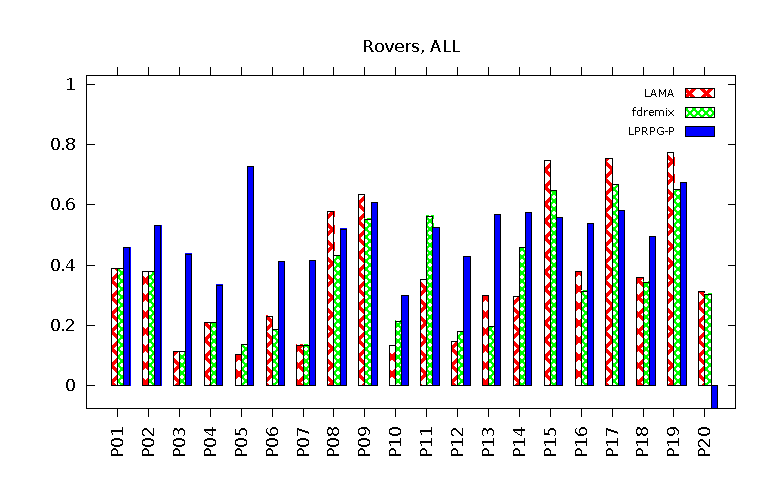
\includegraphics[width=8.5cm]{histogrammi/histogram_rovers_ALL_PERCENTAGE_COST.eps}
\caption{Rovers}
\label{lst:file1}
\end{subfigure}
% &
\\
% TPP ALL HISTOGRAM
\begin{subfigure}[b]{\linewidth}
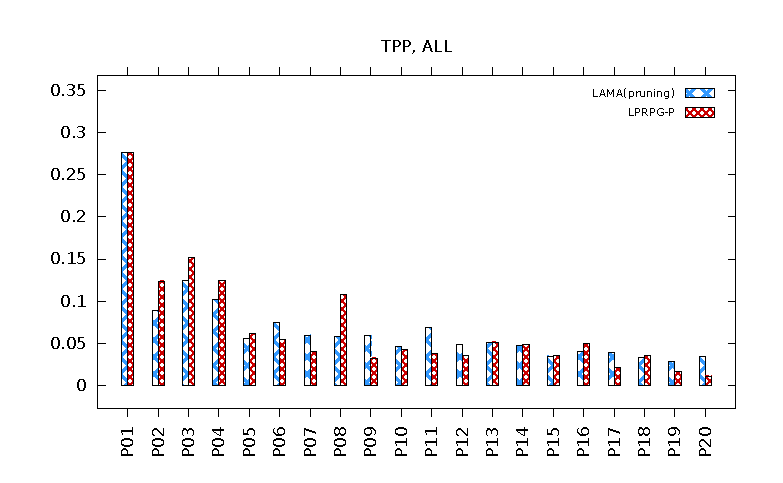
\includegraphics[width=8.5cm]{histogrammi/histogram_tpp_ALL_PERCENTAGE_COST.eps}
\caption{TPP}
\label{lst:file2}
\end{subfigure} \\
% TRUCKS
\begin{subfigure}[b]{\linewidth}
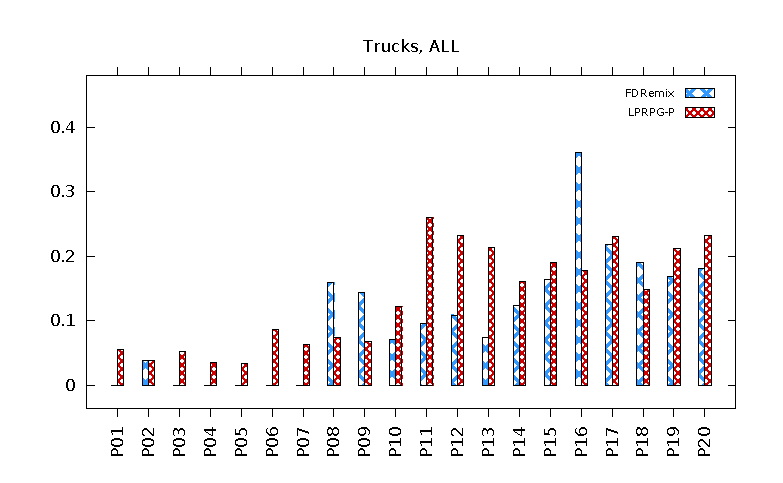
\includegraphics[width=8.5cm]{histogrammi/histogram_trucks_ALL_PERCENTAGE_COST.eps}
\caption{Trucks}
\label{lst:file3}
\end{subfigure}

\end{figure}

\begin{figure}[htb] \ContinuedFloat
% OPENSTACKS
\begin{subfigure}[b]{\linewidth}
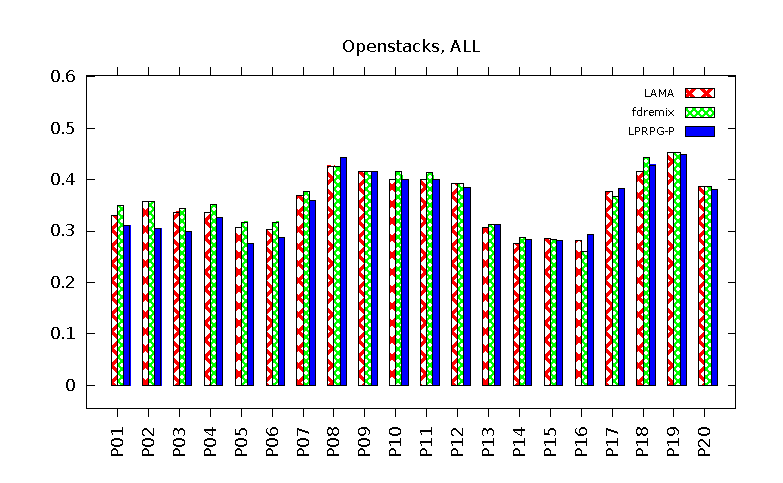
\includegraphics[width=8.5cm]{histogrammi/histogram_openstacks_ALL_PERCENTAGE_COST.eps}
\caption{Openstacks}
\label{lst:file4}
\end{subfigure}
\\
% \end{tabular}
% \begin{tabular}{c}
% STORAGE
\begin{subfigure}[b]{\linewidth}
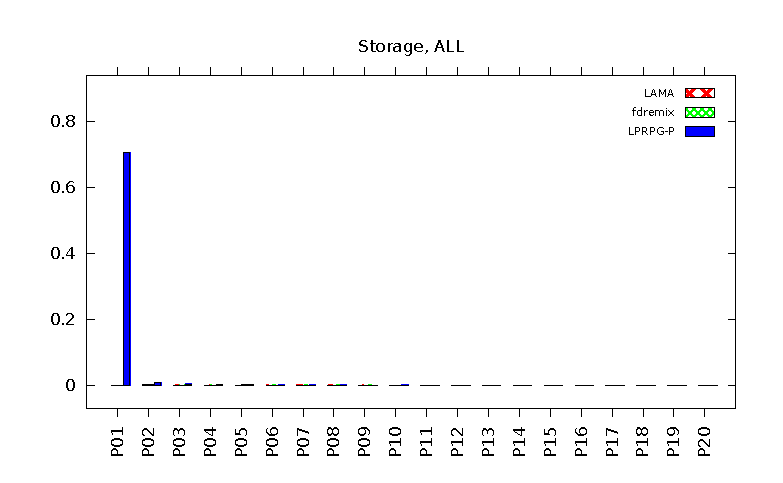
\includegraphics[width=8.5cm]{histogrammi/histogram_preprocessed-storage_ALL_PERCENTAGE_COST.eps}
\caption{Storage}
\label{lst:file5}
\end{subfigure}
\\

% \end{tabular}

% \captionsetup{font=scriptsize}
\caption{Quality Comparison using $\alpha_{\textit{cost}}$ for each domain. Each bar represents the $\alpha_{\textit{cost}}$ of the best plan produced by the considered planner. The negative bar represents an instance which has not been solved or that has no preferences of that kind. From the top to bottom we have provided the results about $\alpha_{\textit{cost}}$ calculated considering each kind of preferences for Rovers, TPP, Trucks, Openstacks and Storage.}
\label{eps:histogram_histograms_ALL_PERCENTAGE_COST}
% \stepcounter{lstlisting}
% \setcounter{figure}{\thetmp}
\end{figure}


% RESTANTI HISTOGRAMMI COMMENTATI

% %%%%%%%%%%%%%%%%%%
% % ROVERS results %
% %%%%%%%%%%%%%%%%%%
% \begin{figure}[H]
% \centering
% \captionof*{table}{Rovers}
% \begin{tabular}{cc}

% \begin{subfigure}{\linewidth}
% 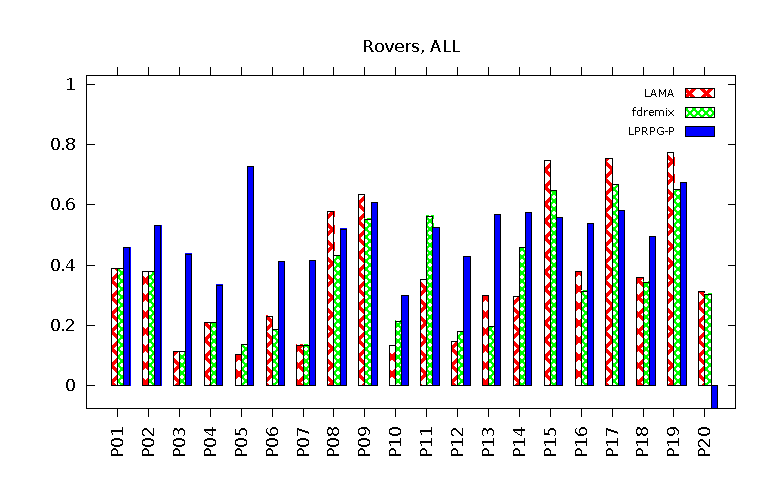
\includegraphics[width=8.5cm]{histogrammi/histogram_rovers_ALL_PERCENTAGE_COST.eps}
% \caption{All}
% \label{lst:file1}
% \end{subfigure}
% &
% \begin{subfigure}{\linewidth}
% 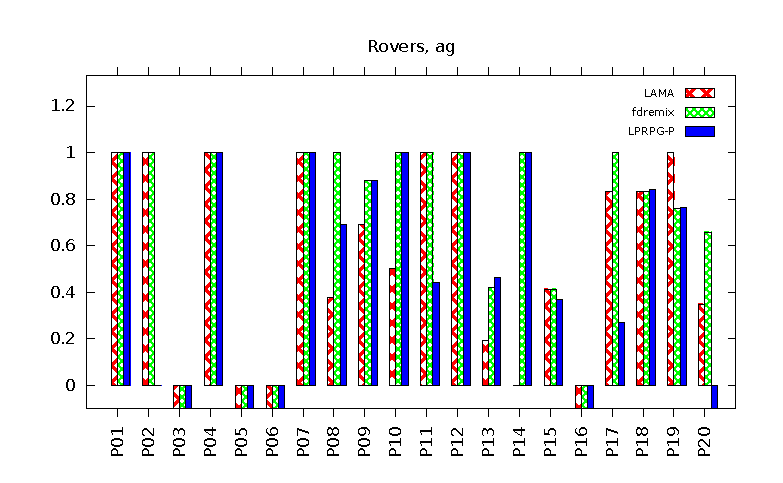
\includegraphics[width=8.5cm]{histogrammi/histogram_rovers_ag_PERCENTAGE_COST.eps}
% \caption{$\mathcal{A}$}
% \label{lst:file2}
% \end{subfigure} \\
% \begin{subfigure}{\linewidth}
% 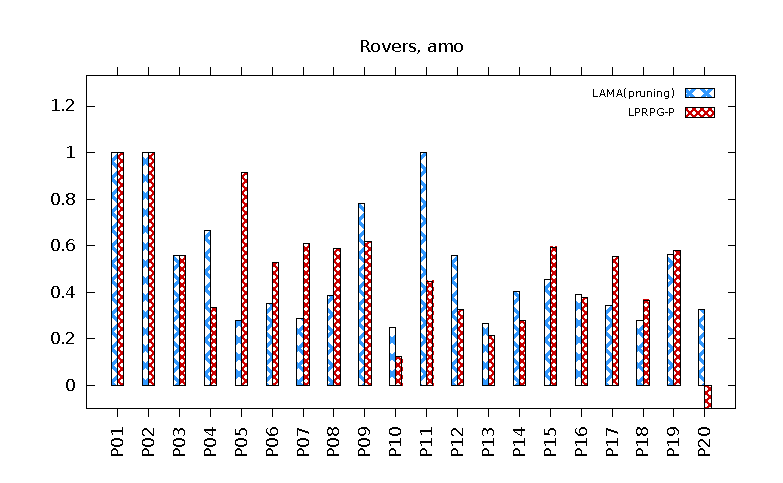
\includegraphics[width=8.5cm]{histogrammi/histogram_rovers_amo_PERCENTAGE_COST.eps}
% \caption{$\mathcal{AO}$}
% \label{lst:file1}
% \end{subfigure}
% &
% \begin{subfigure}{\linewidth}
% 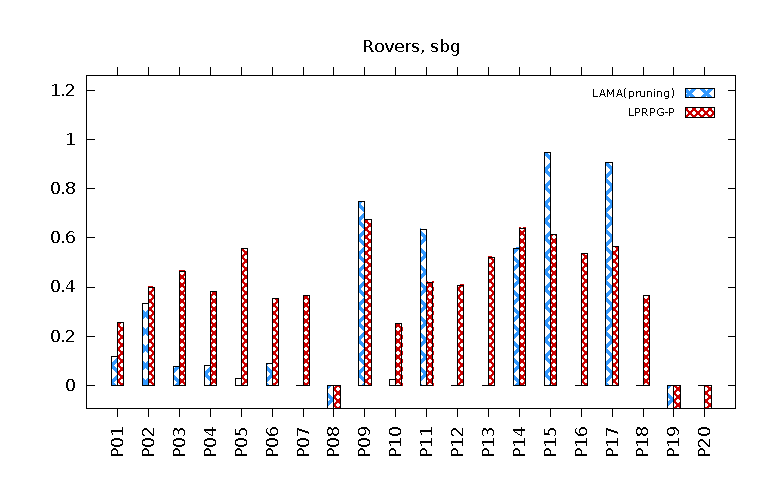
\includegraphics[width=8.5cm]{histogrammi/histogram_rovers_sbg_PERCENTAGE_COST.eps}
% \caption{$\mathcal{SB}$}
% \label{lst:file2}
% \end{subfigure} \\

% \end{tabular}

% \begin{tabular}{c}

% \begin{subfigure}{\linewidth}
% 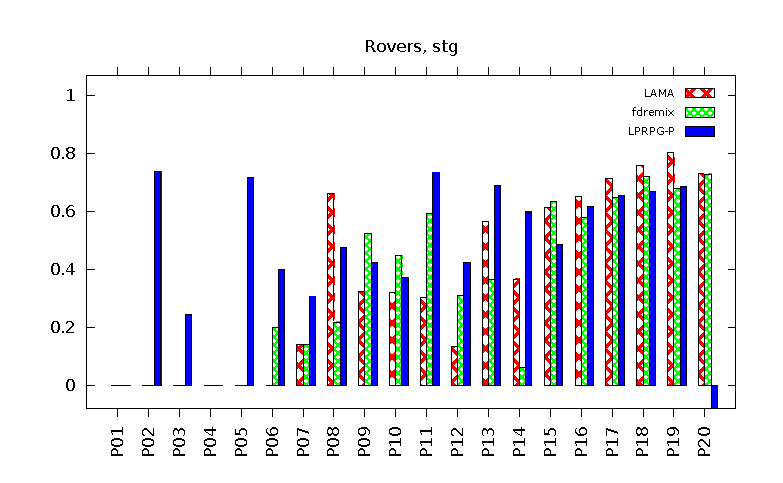
\includegraphics[width=8.5cm]{histogrammi/histogram_rovers_stg_PERCENTAGE_COST.eps}
% \caption{$\mathcal{ST}$}
% \label{lst:file2}
% \end{subfigure} \\

% \end{tabular}


% % \captionsetup{font=scriptsize}
% \caption{Domain: Rovers. Black: LAMA, Grey: IBaCoP2, Light-Grey: LPRPG-P. Each bar represents the $\alpha_{\textit{cost}}$ of the best plan produced by the considered planner. The negative bar represents an instance which has not been solved or that has no preferences of that kind. From left to right we have provided the results about the $\alpha_{\textit{cost}}$ calculated considering each kind of preferences, always, at-most-once, sometime-before and sometime preferences.}
% \label{eps:histogram_histograms_rovers.eps}

% \end{figure}

% %%%%%%%%%%%%%%%
% % TPP results %
% %%%%%%%%%%%%%%%
\begin{figure}[]
\centering

% \begin{tabular}{cc}

% \begin{subfigure}{\linewidth}
% 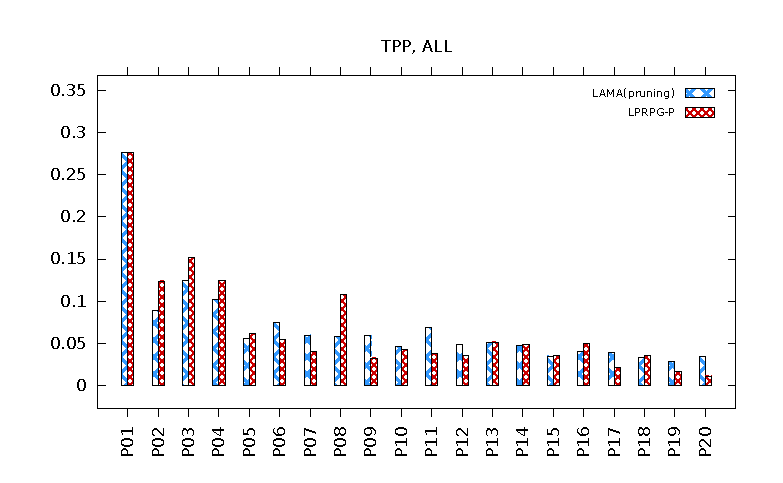
\includegraphics[width=8.5cm]{histogrammi/histogram_tpp_ALL_PERCENTAGE_COST.eps}
% \caption{All}
% \label{lst:tpp:all}
% \end{subfigure}
% &
% \begin{subfigure}{\linewidth}
% 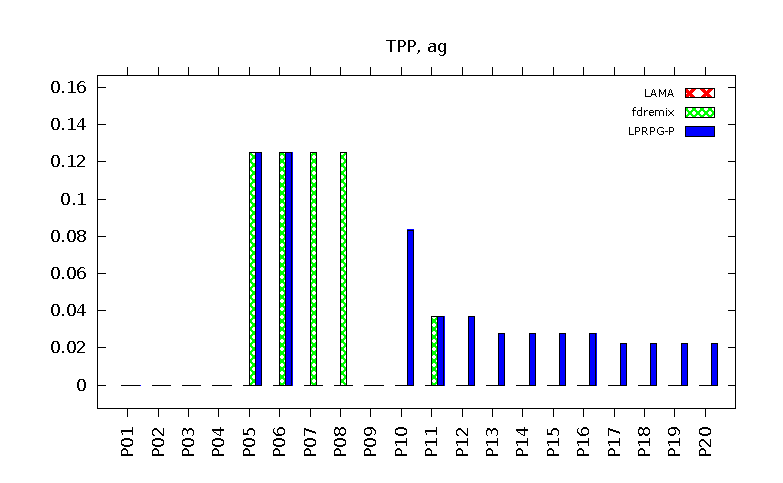
\includegraphics[width=8.5cm]{histogrammi/histogram_tpp_ag_PERCENTAGE_COST.eps}
% \caption{$\mathcal{A}$}
% \label{lst:tpp:ag}
% \end{subfigure}
% \\
\begin{subfigure}{\linewidth}
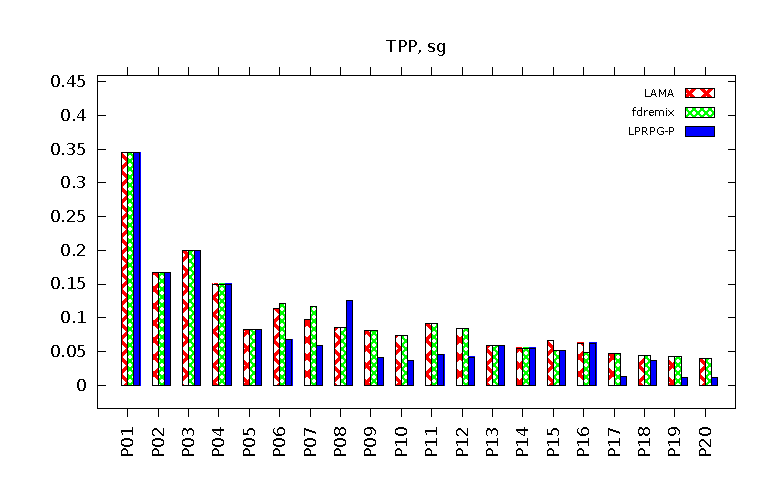
\includegraphics[width=8.5cm]{histogrammi/histogram_tpp_sg_PERCENTAGE_COST.eps}
\caption{$\mathcal{SG}$}
\label{lst:tpp:sg}
\end{subfigure}
% &
% \begin{subfigure}{\linewidth}
% 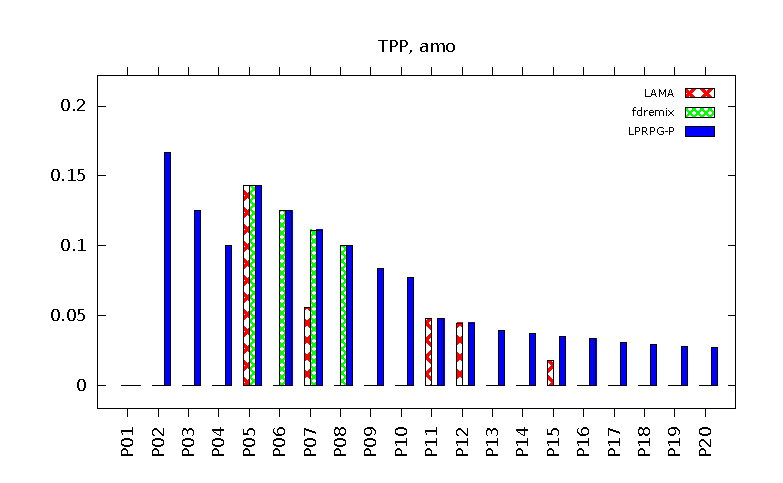
\includegraphics[width=8.5cm]{histogrammi/histogram_tpp_amo_PERCENTAGE_COST.eps}
% \caption{$\mathcal{AO}$}
% \label{lst:tpp:amo}
% \end{subfigure}
% \\
% \begin{subfigure}{\linewidth}
% 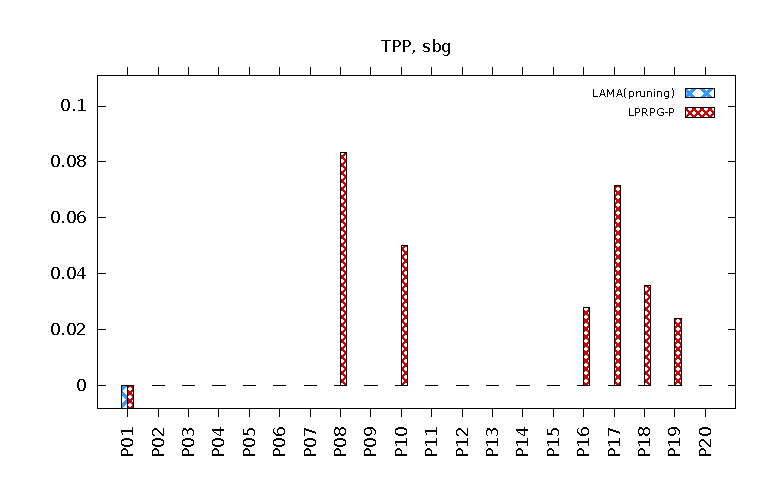
\includegraphics[width=8.5cm]{histogrammi/histogram_tpp_sbg_PERCENTAGE_COST.eps}
% \caption{$\mathcal{SB}$}
% \label{lst:tpp:sbg}
% \end{subfigure}
% &
\begin{subfigure}{\linewidth}
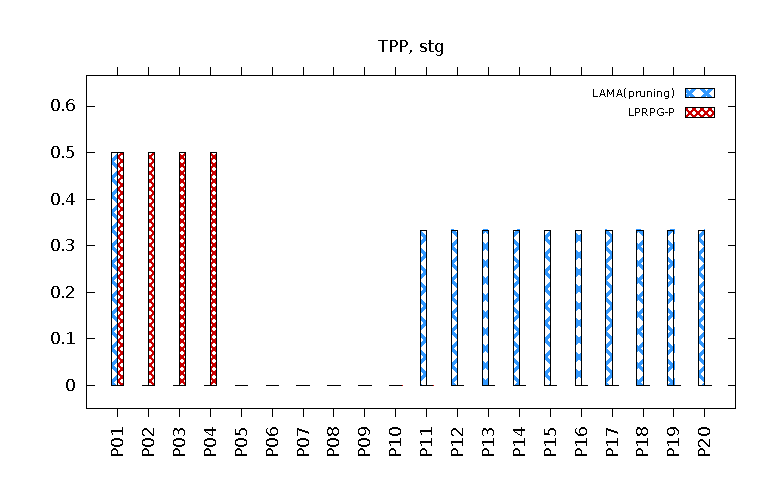
\includegraphics[width=8.5cm]{histogrammi/histogram_tpp_stg_PERCENTAGE_COST.eps}
\caption{$\mathcal{ST}$}
\label{lst:tpp:st}
\end{subfigure}

% \end{tabular}

% \captionsetup{font=scriptsize}
\caption{Each bar represents the $\alpha_{\textit{cost}}$ of the best plan produced by the considered planner. The negative bar represents an instance which has not been solved or that has no preferences of that kind. From left to right we have provided the results about the $\alpha_{\textit{cost}}$ calculated considering each kind of preferences, always, at-end (or soft goals), at-most-once, sometime-before and sometime preferences.}
\label{eps:histogram_histograms_tpp.eps.sg}

\end{figure}

% %%%%%%%%%%
% % TRUCKS %
% %%%%%%%%%%
% \begin{figure}[H]
% \centering

% \begin{tabular}{cc}

% % ROVERS ALL HISTOGRAM
% \begin{subfigure}{\linewidth}
% 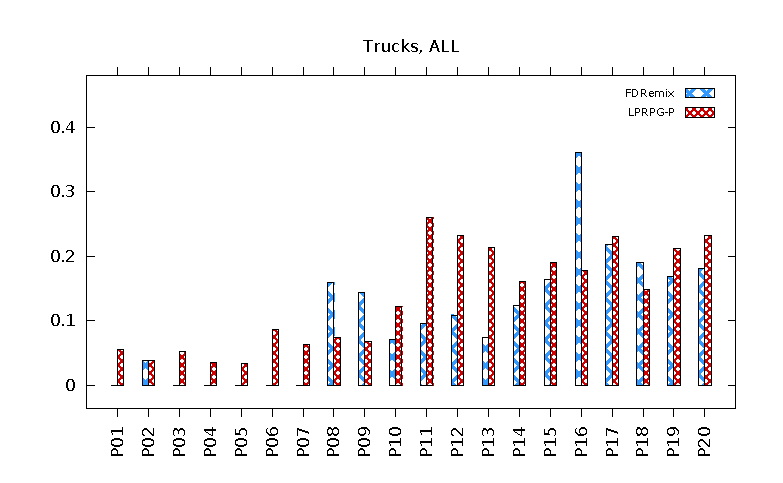
\includegraphics[width=8.5cm]{histogrammi/histogram_trucks_ALL_PERCENTAGE_COST.eps}
% \caption{All}
% \label{lst:file1}
% \end{subfigure}
% &
% % TPP ALL HISTOGRAM
% \begin{subfigure}{\linewidth}
% 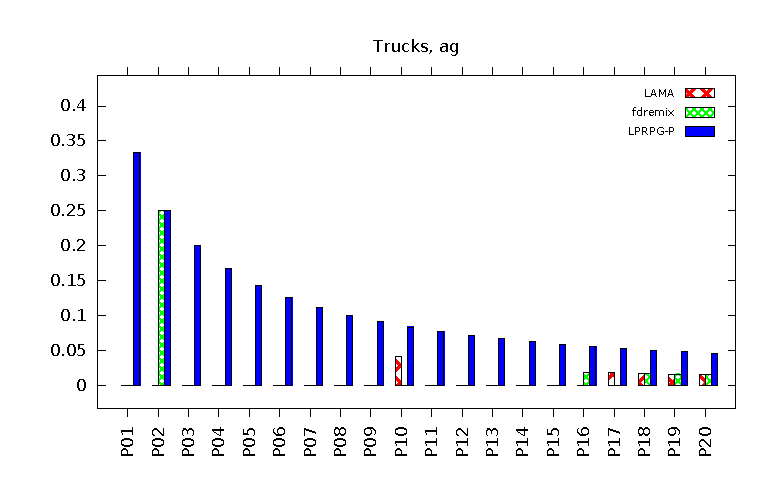
\includegraphics[width=8.5cm]{histogrammi/histogram_trucks_ag_PERCENTAGE_COST.eps}
% \caption{$\mathcal{A}$}
% \label{lst:file2}
% \end{subfigure} \\
% % TRUCKS
% \begin{subfigure}{\linewidth}
% 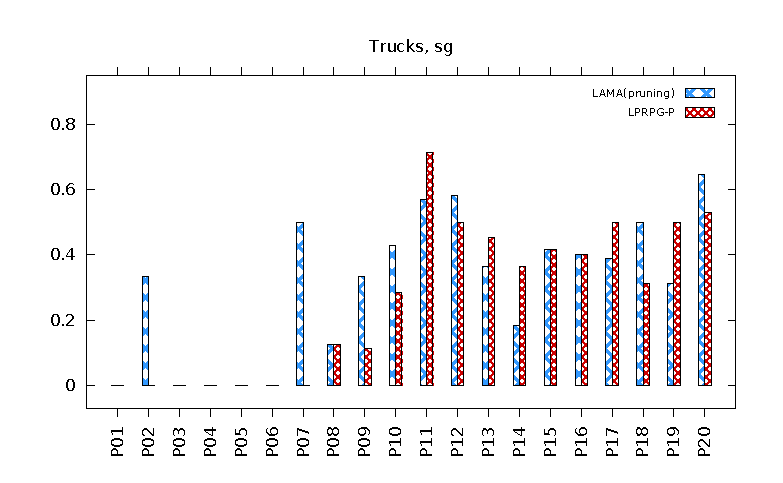
\includegraphics[width=8.5cm]{histogrammi/histogram_trucks_sg_PERCENTAGE_COST.eps}
% \caption{$\mathcal{SG}$}
% \label{lst:file1}
% \end{subfigure}
% &
% % OPENSTACKS
% \begin{subfigure}{\linewidth}
% 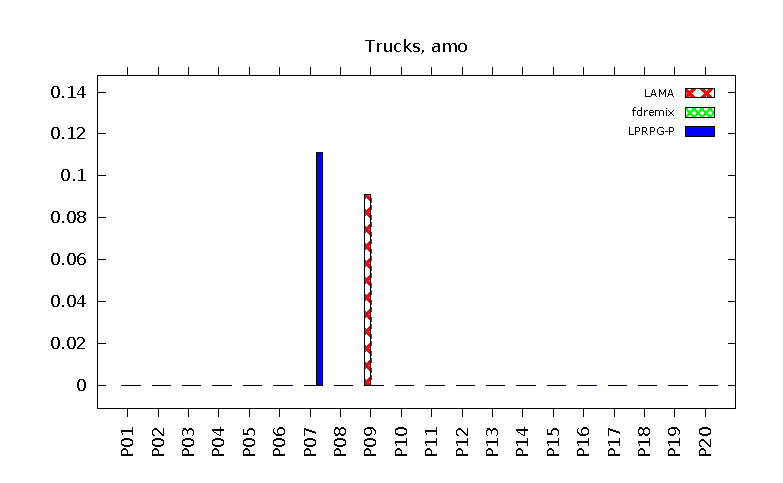
\includegraphics[width=8.5cm]{histogrammi/histogram_trucks_amo_PERCENTAGE_COST.eps}
% \caption{$\mathcal{AO}$}
% \label{lst:file2}
% \end{subfigure} \\

% \end{tabular}

% \begin{tabular}{c}
% % STORAGE
% \begin{subfigure}{\linewidth}
% 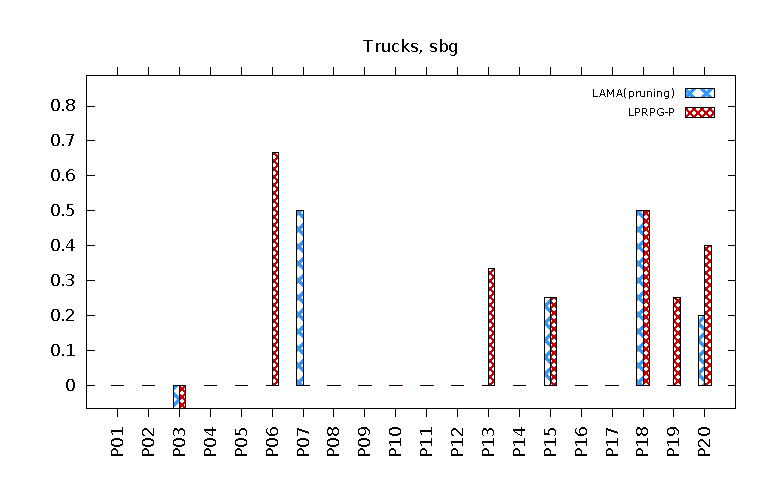
\includegraphics[width=8.5cm]{histogrammi/histogram_trucks_sbg_PERCENTAGE_COST.eps}
% \caption{$\mathcal{SB}$}
% \label{lst:file2}
% \end{subfigure} \\

% \end{tabular}

% % \captionsetup{font=scriptsize}
% \caption{Domain: Trucks. Black: LAMA, Grey: IBaCoP2, Light-Grey: LPRPG-P. Each bar represents the $\alpha_{\textit{cost}}$ of the best plan produced by the considered planner. The negative bar represents an instance which has not been solved or that has no preferences of that kind. From left to right we have provided the results about the $\alpha_{\textit{cost}}$ calculated considering each kind of preferences, always, at-end (or soft goals), at-most-once, sometime-before preferences.}
% \label{eps:histogram_histograms_trucks.eps}

% \end{figure}

% %%%%%%%%%%%%%%
% % OPENSTACKS %
% %%%%%%%%%%%%%%
% \begin{figure}[H]
% \centering

% \begin{tabular}{cc}

% \begin{subfigure}{\linewidth}
% 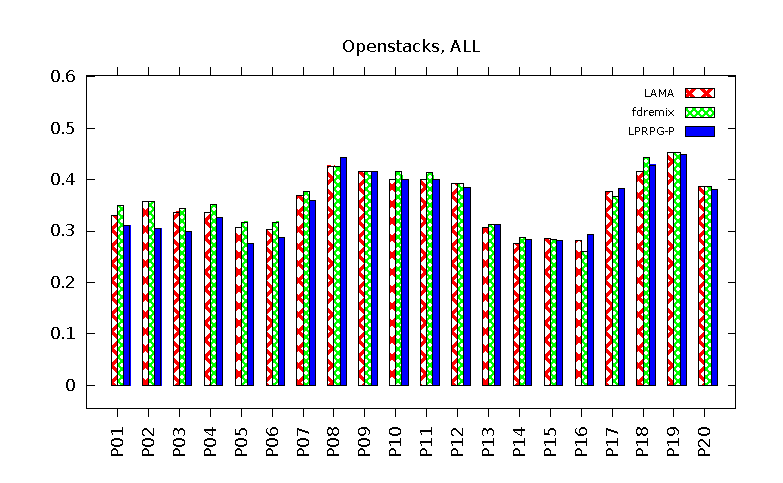
\includegraphics[width=8.5cm]{histogrammi/histogram_openstacks_ALL_PERCENTAGE_COST.eps} 
% \caption{All}
% \label{lst:os:all}
% \end{subfigure}
% &

% \begin{subfigure}{\linewidth}
% 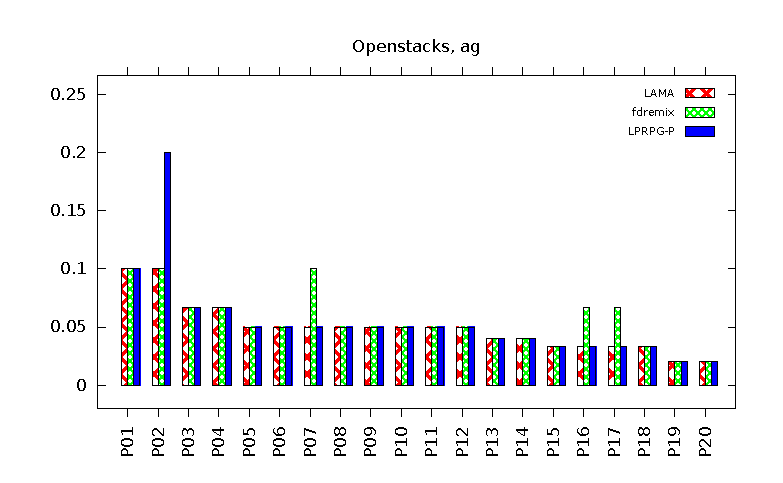
\includegraphics[width=8.5cm]{histogrammi/histogram_openstacks_ag_PERCENTAGE_COST.eps}
% \caption{$\mathcal{A}$}
% \label{lst:os:ag}
% \end{subfigure}
% \\

% \end{tabular}

% \begin{tabular}{c}

% \begin{subfigure}{\linewidth}
% 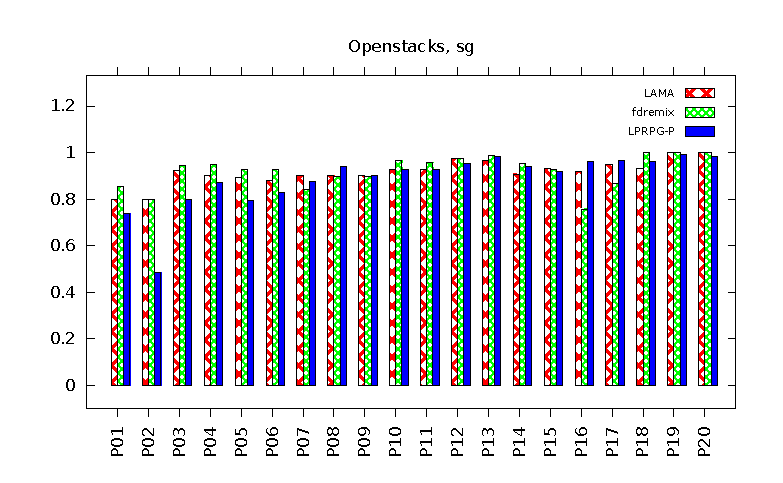
\includegraphics[width=8.5cm]{histogrammi/histogram_openstacks_sg_PERCENTAGE_COST.eps}
% \caption{$\mathcal{SG}$}
% \label{lst:os:sg}
% \end{subfigure}

% \end{tabular}

% % \captionsetup{font=scriptsize}
% \caption{Domain: Openstacks. Black: LAMA, Grey: IBaCoP2, Light-Grey: LPRPG-P. Each bar represents the $\alpha_{\textit{cost}}$ of the best plan produced by the considered planner. The negative bar represents an instance which has not been solved or that has no preferences of that kind. From left to right we have provided the results about the $\alpha_{\textit{cost}}$ calculated considering each kind of preferences, always and at end (or soft goals) preferences.}
% \label{eps:histogram_histograms_openstacks.eps}

% \end{figure}


% %%%%%%%%%%%%%%%%%%%
% % STORAGE results %
% %%%%%%%%%%%%%%%%%%%
% \begin{figure}[H]
% \centering

% \begin{tabular}{cc}

% \begin{subfigure}{\linewidth}
% 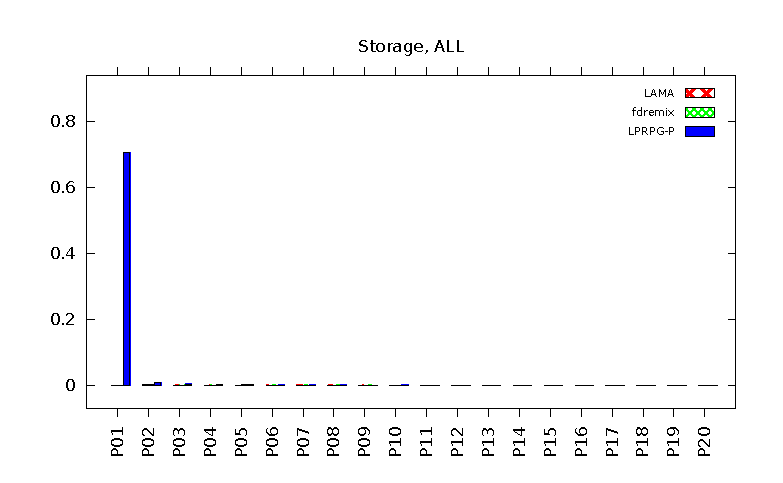
\includegraphics[width=8.5cm]{histogrammi/histogram_preprocessed-storage_ALL_PERCENTAGE_COST.eps}
% \caption{All}
% \label{lst:file1}
% \end{subfigure}
% &
% \begin{subfigure}{\linewidth}
% 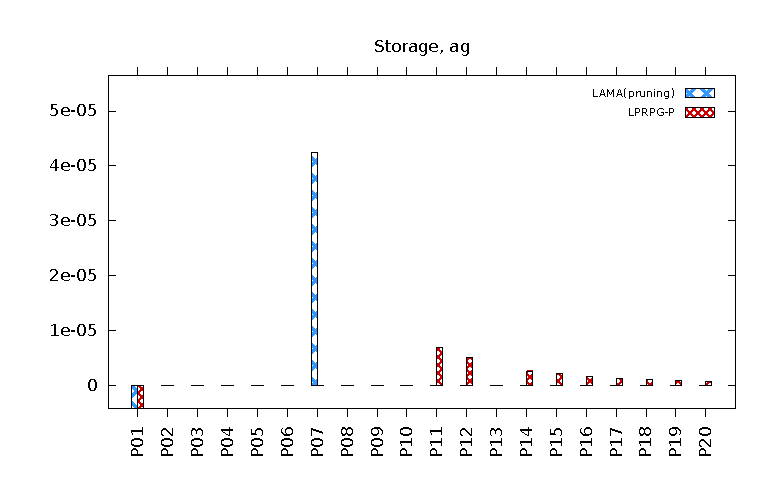
\includegraphics[width=8.5cm]{histogrammi/histogram_preprocessed-storage_ag_PERCENTAGE_COST.eps}
% \caption{$\mathcal{A}$}
% \label{lst:file2}
% \end{subfigure} \\
% \begin{subfigure}{\linewidth}
% 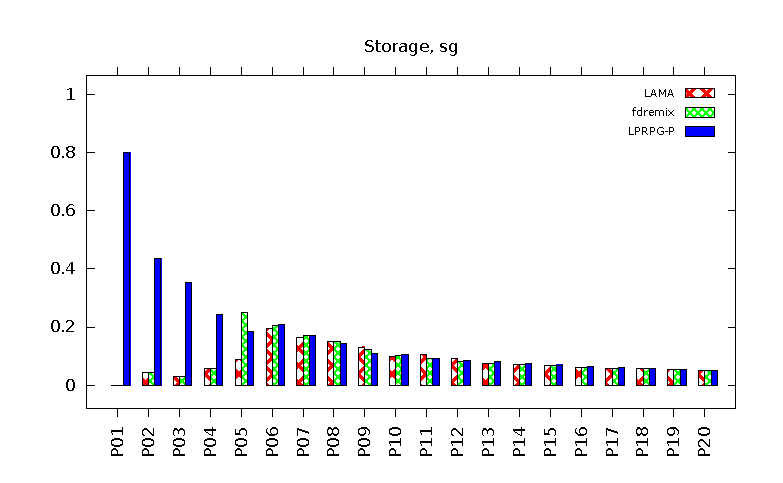
\includegraphics[width=8.5cm]{histogrammi/histogram_preprocessed-storage_sg_PERCENTAGE_COST.eps}
% \caption{$\mathcal{SG}$}
% \label{lst:file1}
% \end{subfigure}
% &
% \begin{subfigure}{\linewidth}
% 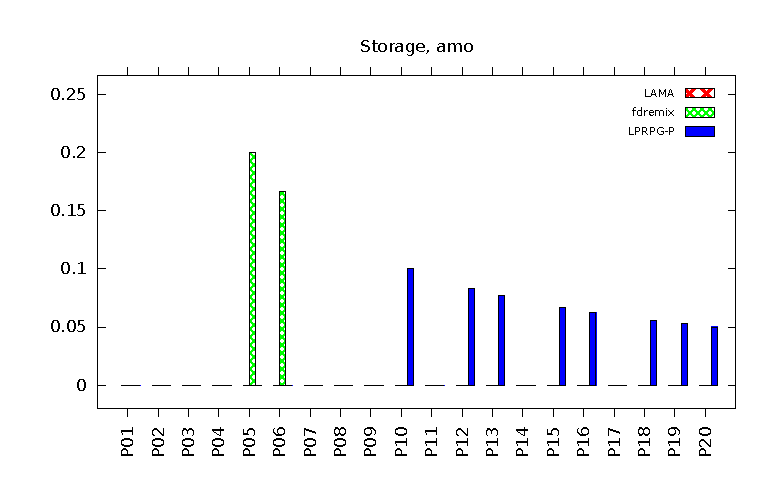
\includegraphics[width=8.5cm]{histogrammi/histogram_preprocessed-storage_amo_PERCENTAGE_COST.eps}
% \caption{$\mathcal{AO}$}
% \label{lst:file2}
% \end{subfigure}
% \\
% \begin{subfigure}{\linewidth}
% 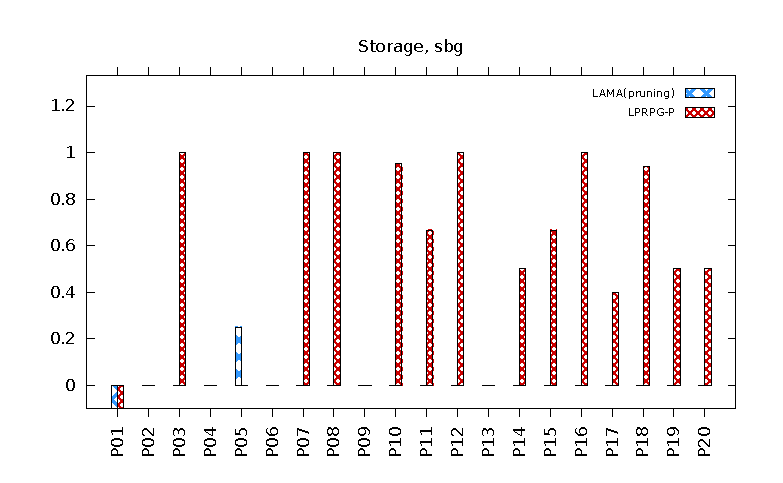
\includegraphics[width=8.5cm]{histogrammi/histogram_preprocessed-storage_sbg_PERCENTAGE_COST.eps}
% \caption{$\mathcal{SB}$}
% \label{lst:file2}
% \end{subfigure}
% &
% \begin{subfigure}{\linewidth}
% 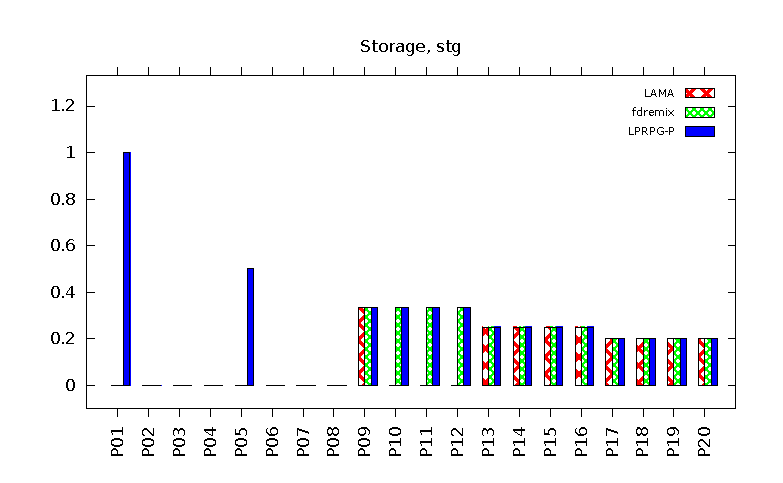
\includegraphics[width=8.5cm]{histogrammi/histogram_preprocessed-storage_stg_PERCENTAGE_COST.eps}
% \caption{$\mathcal{ST}$}
% \label{lst:file2}
% \end{subfigure}

% \end{tabular}


% % \captionsetup{font=scriptsize}
% \caption{Domain: Storage. Black: LAMA, Grey: IBaCoP2, Light-Grey: LPRPG-P. Each bar represents the $\alpha_{\textit{cost}}$ of the best plan produced by the considered planner. The negative bar represents an instance which has not been solved or that has no preferences of that kind. From left to right we have provided the results about the $\alpha_{\textit{cost}}$ calculated considering each kind of preferences, always, at-end (or soft goals), at-most-once, sometime-before and sometime preferences.}
% \label{eps:histogram_histograms_storage.eps}

% \end{figure}


\subsection{Optimal Planning Results}

Similarly to what to what has been done in \cite{nebel2018}, we have tested our scheme
using some admissible heuristics which are $h^\text{blind}$, which assign 1 to all states except
for goal states to which assign 0, the maximum heuristic $h^\text{max}$, the merge and shrink heuristic $h^{\text{M\&S}}$, and the canonical pattern database heuristic $h^{\text{cpdb}}$ \cite{{haslum2007domain}}.
These heuristitcs guarantee the optimality of the solution found. Starting from the IPC5 domains,
we generated, similar to what was done \cite{nebel2018},
simpler instances by randomly sampling subsets of the soft trajectory constraints. Starting
from each instance we have generated five new instances with 1\%, 5\%, 10\%, 20\% and 40\% of
the (grounded) soft trajectory constraints while the hard goals have remained unchanged.

Since we do not have the instances that have been used in the aforementioned paper,
we have generated, for each percentage of sampling preferences (except for 100 \%), 3 sampled
instances in order to average the obtained results and be able to compare with their
results. 
All our experiments
were conducted on a 2.00GHz Core Intel(R) Xeon(R) CPU E5-2620 machine with CPU-time
and memory limits of 30 minutes and 8GiB, respectively, while the experiments 
reported in \cite{nebel2018} are conducted on a
Intel(R) Xeon(R) E5-2650v2 2.60GHz processors with 64GiB with one hour of CPU-time
for the search and then our approach is penalized.

The results about this experiment and the comparison with the automata approach
are shown Table \ref{coverage_admissible_heuristics}. The results
inherent to Openstacks have been excluded because it was not possible to find optimal
plans even for the simplest instances. 


\begin{table}[]
\scriptsize
\centering
\begin{tabular}{|c||c|c||c|c||c|c||c|c||}
\hline 
\multirow{2}{*}{DOMINO} & \multicolumn{2}{c||}{$h^{\text{blind}}$} & \multicolumn{2}{c||}{$h^{\text{max}}$} & \multicolumn{2}{c||}{$h^{\text{m\&s}}$} & \multicolumn{2}{c||}{$h^{\text{cpdb}}$} \\ \cline{2-9}
& Nebel& Our & Nebel & Our& Nebel& Our& Nebel & Our \\ \hline
% Storage & --- &  --- &  --- &  --- &  --- &  --- &  --- &  --- \hline
% Domain & $h^{\text{blind}}$ & $h^{\text{max}}$ & $h^{\text{m\&s}}$ & $h^{\text{cpdb}}$\\ \hline 
Storage & 24.78 & 57.0 & 29.2 & 45.0 & 32.50 & 24.0 & 23.10 & 57.0 \\ \hline
Rovers & 17.4 & 24.0 & 41.0 & 25.0 & 16.67 & 26.0 & 15.17 & 23.0 \\ \hline
Trucks & 18.84 & 24.0 & 23.19 & 25.0 & n/a & 25.0 & n/a & 25 \\ \hline
TPP & --- & 47.0 & --- & 45.0 & --- & 47.0 & -- & 40.0 \\ \hline

%  % & ---& ---& --- & ---\\ \hline
% \multirow{2}{*}{Rovers} & 23.0& 23.0& 23.0 &\\  \cline{2-5} 
%  % & ---& ---& --- & ---\\ \hline
% \multirow{2}{*}{TPP} & 36.0& 33.0& 35.0 &\\  \cline{2-5} 
%  % & ---& ---& --- & ---\\ \hline
% \multirow{2}{*}{Trucks} & 23.0& 28.0& 23.0 &\\  \cline{2-5} 
%  % & ---& ---& --- & ---\\ \hline
% \multirow{2}{*}{TOTAL} & 33.0& 31.0& 26.0 &\\ \cline{2-5}  
 % & ---& ---& --- & ---\\ \hline


\end{tabular}
\caption{Coverage of our and Nebel compilation scheme on the IPC5 benchmarks set with
additional instances with random sampled soft-trajectory constraints, A*
search for optimal solution. Our results concerning the sampled instances are averaged.}
\label{coverage_admissible_heuristics}
\end{table}


\section{Conclusions}



\bibliographystyle{plain}
\bibliography{biblio.bib}
\end{document}
